\begin{minipage}[t]{0.49\linewidth}\centering
{\color{black}\normalsize\bfseries LLM + RAG}\par\smallskip
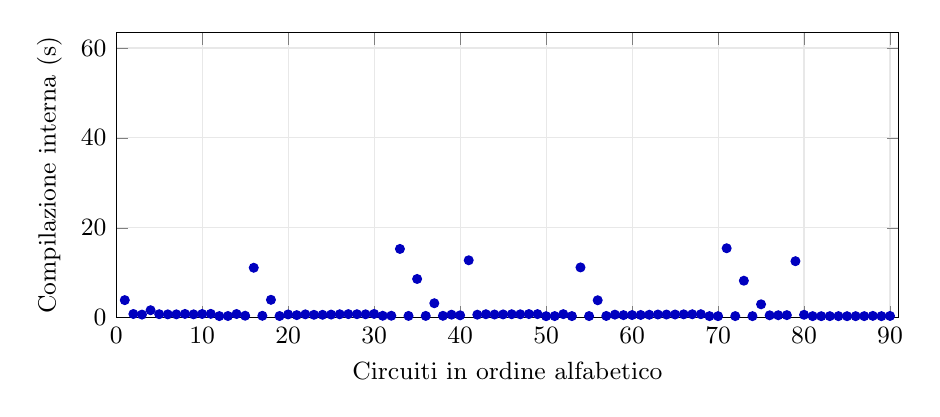
\begin{tikzpicture}\begin{axis}[width=0.95\linewidth,height=5.2cm,grid=major,grid style={gray!18},tick label style={font=\small},label style={font=\small},scaled ticks=false,/pgf/number format/use comma,unbounded coords=discard,xlabel={Circuiti in ordine alfabetico},ylabel={Compilazione interna (s)},xmin=0,xmax=91,ymin=0,ymax=63.37173401028009,]
\addplot[color=blue!75!black,mark=*,mark size=1.6pt,only marks] coordinates {(1,3.922640659000024) (2,0.8393507979999413) (3,0.7046502950000786) (4,1.6770110780000778) (5,0.7918471919999774) (6,0.7587581049999699) (7,0.7601908209999237) (8,0.8547360070000423) (9,0.7606678759999568) (10,0.8392648290000579) (11,0.8734190100000205) (12,0.37290141800008314) (13,0.3913027799999327) (14,0.8351566779999757) (15,0.4550175520000721) (16,11.123879788999943) (17,0.4380465850000519) (18,3.992816368999911) (19,0.38925532200005364) (20,0.7426763109999683) (21,0.5887380310000481) (22,0.7587382599999728) (23,0.6603850770000008) (24,0.6617466129998775) (25,0.7081877670000267) (26,0.7795202239999526) (27,0.8136023179999938) (28,0.7914576260000104) (29,0.769515303000162) (30,0.8537167019999288) (31,0.44674727900019207) (32,0.4523840970000492) (33,15.311303501999873) (34,0.41094514699989304) (35,8.631899993999923) (36,0.41209178500002963) (37,3.2298512810000375) (38,0.4384583149999344) (39,0.6857099580001886) (40,0.5492403670000385) (41,12.785060631000079) (42,0.6850940659999196) (43,0.7859162770000694) (44,0.7222933319999356) (45,0.7471961999999621) (46,0.7873398270000962) (47,0.7743332150000697) (48,0.8262390660001984) (49,0.8156420410000464) (50,0.3567695739998271) (51,0.3785179630001494) (52,0.8063989469999342) (53,0.37487343499992676) (54,11.197072114000093) (55,0.37784067500001584) (56,3.8923991629999364) (57,0.40457731100013916) (58,0.69529813500003) (59,0.5903850220001914) (60,0.606412144999922) (61,0.6208897090000391) (62,0.6700452000000041) (63,0.7226054050001949) (64,0.7188779420002902) (65,0.7248702910001157) (66,0.7621132310000576) (67,0.7802756340001906) (68,0.7916319239998302) (69,0.3661621819996981) (70,0.3611586229999375) (71,15.462561265000204) (72,0.37400757700015674) (73,8.241070083000068) (74,0.36320157299996936) (75,2.9943760850001127) (76,0.5471323619999566) (77,0.5647790210000494) (78,0.5864484290000291) (79,12.58391740900015) (80,0.663703777000137) (81,0.36373396299995875) (82,0.35435010899982444) (83,0.36207918299987796) (84,0.3632980900001712) (85,0.351774118999856) (86,0.35865022600000884) (87,0.3639074550001169) (88,0.421760909999648) (89,0.36172354300015286) (90,0.40446023100003003)};
\end{axis}\end{tikzpicture}
\end{minipage}
\hfill\begin{minipage}[t]{0.49\linewidth}\centering
{\color{black}\normalsize\bfseries LLM no RAG}\par\smallskip
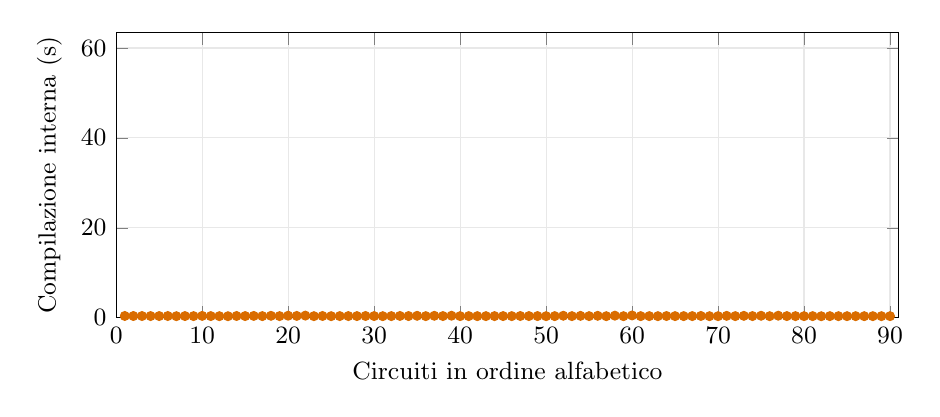
\begin{tikzpicture}\begin{axis}[width=0.95\linewidth,height=5.2cm,grid=major,grid style={gray!18},tick label style={font=\small},label style={font=\small},scaled ticks=false,/pgf/number format/use comma,unbounded coords=discard,xlabel={Circuiti in ordine alfabetico},ylabel={Compilazione interna (s)},xmin=0,xmax=91,ymin=0,ymax=63.37173401028009,]
\addplot[color=orange!85!black,mark=*,mark size=1.6pt,only marks] coordinates {(1,0.39856766000048083) (2,0.3894500270007484) (3,0.3878795929995249) (4,0.38087481200000184) (5,0.38183666999975685) (6,0.3891634380006508) (7,0.353121246000228) (8,0.3802336409999043) (9,0.3708955749998495) (10,0.4171618150003269) (11,0.37559209699975327) (12,0.35608952899929136) (13,0.3484409990005588) (14,0.39579487399987556) (15,0.3784480160002204) (16,0.4103624930003207) (17,0.37063956300062273) (18,0.43599960600022314) (19,0.37041646699981357) (20,0.4589222599997811) (21,0.4106656699996165) (22,0.48192376000042714) (23,0.3576416350006184) (24,0.39512368200030323) (25,0.3574532069997076) (26,0.3732635139995182) (27,0.37946867299979203) (28,0.37493053899925144) (29,0.39692710300005274) (30,0.380099290000544) (31,0.3562988490002681) (32,0.37033202099974005) (33,0.40418596700055787) (34,0.381978096000239) (35,0.4352138719996219) (36,0.3650747150004463) (37,0.43895259400051145) (38,0.3802946599998904) (39,0.45752646600067237) (40,0.3654964540000947) (41,0.3692337320007937) (42,0.36406184299994493) (43,0.36449802000061027) (44,0.3722121260007043) (45,0.37427836599999864) (46,0.3667212020000079) (47,0.3916249430003518) (48,0.3768832420000763) (49,0.37804813200000353) (50,0.3565321779997248) (51,0.3660862480001015) (52,0.44661850900047284) (53,0.36573968199991214) (54,0.42467922200012254) (55,0.3653824370003349) (56,0.433297369999309) (57,0.3544967580000957) (58,0.46702329799973086) (59,0.35503456100013864) (60,0.515547730000435) (61,0.36361701499936316) (62,0.3673284189999322) (63,0.35930803700011893) (64,0.388070792999315) (65,0.3677844809999442) (66,0.3665622069993333) (67,0.3714018259997829) (68,0.4030254649997005) (69,0.35376317699956417) (70,0.35611168299965357) (71,0.42456369000046834) (72,0.36781271700056095) (73,0.4278093050006646) (74,0.37563372300064657) (75,0.44499932400049147) (76,0.35578333999910683) (77,0.459806328999548) (78,0.37398189899977297) (79,0.3698004410007343) (80,0.36258662000000186) (81,0.3649251050001112) (82,0.3445493050003279) (83,0.3623610169997846) (84,0.35891357499986043) (85,0.3577669650003372) (86,0.360136247999435) (87,0.35658640899964666) (88,0.3578440440005579) (89,0.3579667920002976) (90,0.36155479499939247)};
\end{axis}\end{tikzpicture}
\end{minipage}
\par\vspace{0.25cm}\begin{minipage}[t]{0.49\linewidth}\centering
{\color{black}\normalsize\bfseries MQT Predictor (esplorativo)}\par\smallskip
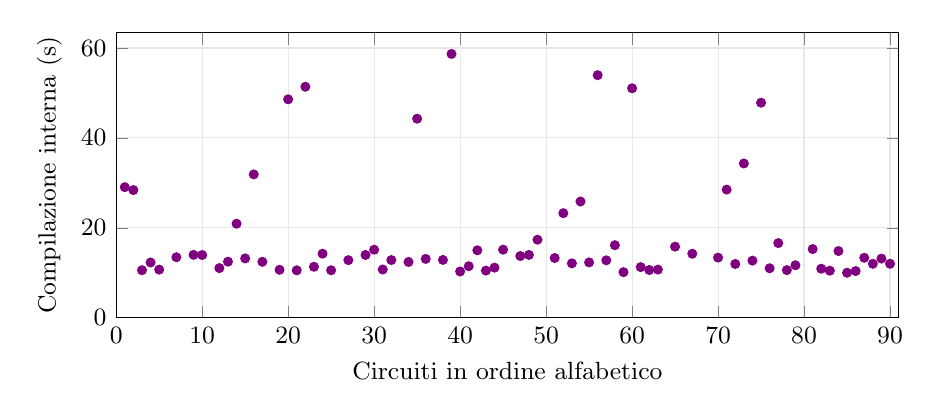
\begin{tikzpicture}\begin{axis}[width=0.95\linewidth,height=5.2cm,grid=major,grid style={gray!18},tick label style={font=\small},label style={font=\small},scaled ticks=false,/pgf/number format/use comma,unbounded coords=discard,xlabel={Circuiti in ordine alfabetico},ylabel={Compilazione interna (s)},xmin=0,xmax=91,ymin=0,ymax=63.37173401028009,]
\addplot[color=violet,mark=*,mark size=1.6pt,only marks] coordinates {(1,29.04545764700015) (2,28.404788131000714) (3,10.580301224999857) (4,12.298171126999478) (5,10.710136548999799) (7,13.46831857899997) (9,13.995648036000603) (10,13.9568404190004) (12,11.046051190999606) (13,12.479570741000316) (14,20.919019164999554) (15,13.20193006000045) (16,31.89010690900068) (17,12.451523555000676) (19,10.666202184999747) (20,48.58148154900027) (21,10.555265320000217) (22,51.38309393500003) (23,11.337600489999204) (24,14.25195802000053) (25,10.57099876599932) (27,12.816791924000427) (29,13.967364555999666) (30,15.135588764999738) (31,10.736975141000585) (32,12.834976703000393) (34,12.413282073000119) (35,44.274198884000725) (36,13.09393637300036) (38,12.865539551999973) (39,58.67753149100008) (40,10.292904883999654) (41,11.465563425000255) (42,15.009362568000142) (43,10.4882625070004) (44,11.15379252799994) (45,15.14947319699968) (47,13.734980174000157) (48,13.981275653999546) (49,17.361874193999938) (51,13.290969431999656) (52,23.265268139) (53,12.102298329000405) (54,25.858956707999823) (55,12.3105374200004) (56,53.95442355000068) (57,12.778935396000634) (58,16.140817382000023) (59,10.145003173000077) (60,51.0418089119994) (61,11.264510705000248) (62,10.624853942999835) (63,10.709578565999436) (65,15.81440124800065) (67,14.240807005999159) (70,13.38120404700021) (71,28.50478343800023) (72,11.967408331000115) (73,34.315387833000386) (74,12.709955657000137) (75,47.83186096500049) (76,11.010313199999473) (77,16.60999564300073) (78,10.600887937999687) (79,11.68105580000065) (81,15.28062354099984) (82,10.908657295999546) (83,10.465330631999677) (84,14.837504727000123) (85,10.018181586000537) (86,10.386899993999577) (87,13.3420845189994) (88,12.00558988299963) (89,13.158063541000047) (90,12.010230876000605)};
\end{axis}\end{tikzpicture}
\end{minipage}
\hfill\begin{minipage}[t]{0.49\linewidth}\centering
{\color{black}\normalsize\bfseries Random}\par\smallskip
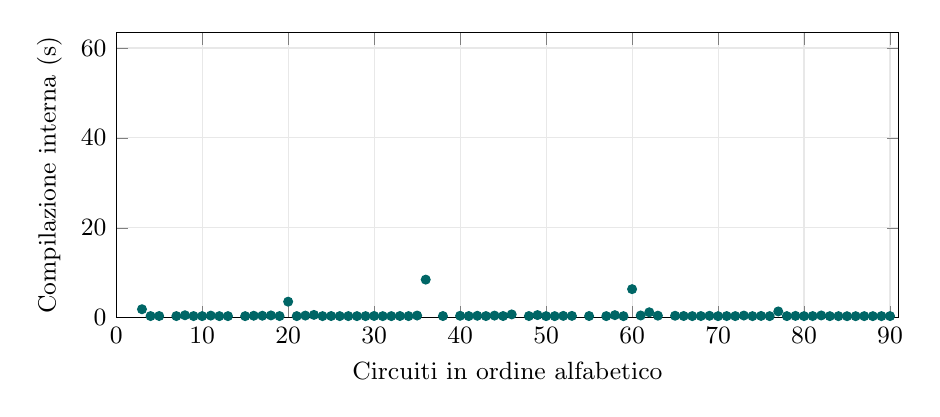
\begin{tikzpicture}\begin{axis}[width=0.95\linewidth,height=5.2cm,grid=major,grid style={gray!18},tick label style={font=\small},label style={font=\small},scaled ticks=false,/pgf/number format/use comma,unbounded coords=discard,xlabel={Circuiti in ordine alfabetico},ylabel={Compilazione interna (s)},xmin=0,xmax=91,ymin=0,ymax=63.37173401028009,]
\addplot[color=teal!80!black,mark=*,mark size=1.6pt,only marks] coordinates {(3,1.8947727129998384) (4,0.38097937800012005) (5,0.39125132300023324) (7,0.3753715010002452) (8,0.5569253720000233) (9,0.38003126600006) (10,0.3699937559999853) (11,0.48226341700001285) (12,0.36479205400019055) (13,0.36512450099962734) (15,0.3647680730000502) (16,0.45153143199968326) (17,0.4539728400000058) (18,0.5209138840000378) (19,0.3778683860000456) (20,3.5796082080000815) (21,0.3702038500000526) (22,0.4871920919999866) (23,0.6368667289998484) (24,0.36953446799998346) (25,0.38980032500012385) (26,0.36995655499958957) (27,0.3713390610000715) (28,0.3666082909999204) (29,0.3693463519998659) (30,0.40334619900022517) (31,0.3656077989999176) (32,0.36778189100004965) (33,0.3915213010000116) (34,0.3740552049998769) (35,0.49729600399996343) (36,8.48329523700022) (38,0.38713507500006017) (40,0.44349320399987846) (41,0.3806287649999831) (42,0.4444854220000707) (43,0.38131653800019194) (44,0.48421729299980143) (45,0.39000403699992603) (46,0.7448169379999854) (48,0.38412940699981846) (49,0.5989112150000437) (50,0.36675724999986414) (51,0.36430993399972067) (52,0.421002020999822) (53,0.4190497209997375) (55,0.3890346349999163) (57,0.3677482510001937) (58,0.5833712290004769) (59,0.361777912999969) (60,6.367271623000306) (61,0.5088414310002918) (62,1.2212644979999823) (63,0.4638370760003454) (65,0.44848613100020884) (66,0.39566836599988164) (67,0.37004400600017107) (68,0.3859510059992317) (69,0.44128319900028146) (70,0.36403058499945473) (71,0.3816446379996705) (72,0.3747417619997577) (73,0.4945746010007497) (74,0.36739298300017253) (75,0.4102263300001141) (76,0.3650787880005737) (77,1.4097335520000343) (78,0.3696311069998046) (79,0.4189125269995202) (80,0.3704458660004093) (81,0.38171458699980576) (82,0.5123590040002455) (83,0.36265141100011533) (84,0.3614604690001215) (85,0.3501107399997636) (86,0.3563025869998455) (87,0.3663512390003234) (88,0.36217110800043884) (89,0.36810680300004606) (90,0.37466254500031937)};
\end{axis}\end{tikzpicture}
\end{minipage}
\par\vspace{0.25cm}\makebox[\linewidth][c]{%
\begin{minipage}[t]{0.49\linewidth}\centering
{\color{black}\normalsize\bfseries LLM + Random RAG (esplorativo)}\par\smallskip
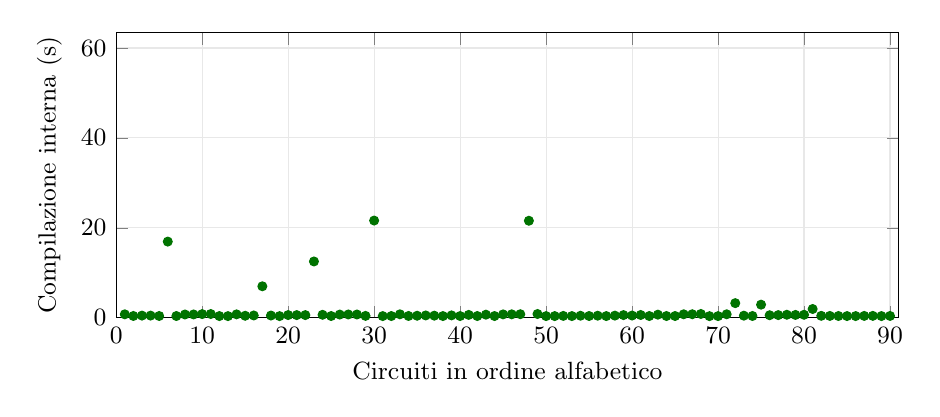
\begin{tikzpicture}\begin{axis}[width=0.95\linewidth,height=5.2cm,grid=major,grid style={gray!18},tick label style={font=\small},label style={font=\small},scaled ticks=false,/pgf/number format/use comma,unbounded coords=discard,xlabel={Circuiti in ordine alfabetico},ylabel={Compilazione interna (s)},xmin=0,xmax=91,ymin=0,ymax=63.37173401028009,]
\addplot[color=green!45!black,mark=*,mark size=1.6pt,only marks] coordinates {(1,0.7654419520000033) (2,0.39918101799997885) (3,0.48334525199999234) (4,0.48390241700002434) (5,0.39598488799998677) (6,16.944056941000042) (7,0.39225186100003384) (8,0.7296082200000455) (9,0.7368781530000206) (10,0.8177768949999518) (11,0.8324213079999936) (12,0.3814725710000175) (13,0.3684814840000854) (14,0.7593186509999441) (15,0.4456982799999878) (16,0.5124717349999628) (17,7.003031924000084) (18,0.497386223000035) (19,0.3704495680000264) (20,0.6015390279999338) (21,0.5942934170000171) (22,0.5948351759999468) (23,12.524759893999999) (24,0.6617285660000789) (25,0.3894276380000292) (26,0.7124159919999329) (27,0.73298945800002) (28,0.7274148700000751) (29,0.4176978739999413) (30,21.621918052999945) (31,0.3738234779998493) (32,0.38681192400008513) (33,0.7713953779998519) (34,0.4019165970000813) (35,0.44916550300013114) (36,0.5178922739999052) (37,0.46686573599981784) (38,0.38299336800014316) (39,0.5306704179999997) (40,0.3837428610002007) (41,0.6386228589999519) (42,0.3886369360000117) (43,0.6868323569999575) (44,0.38625481999997646) (45,0.753456819999883) (46,0.7655064430000493) (47,0.7933496080001987) (48,21.577944659000195) (49,0.8357281180001337) (50,0.374345804000086) (51,0.37429339499999514) (52,0.4155587700001888) (53,0.3775521630000185) (54,0.45562666299997545) (55,0.39125921599998037) (56,0.4596233449999545) (57,0.38035707500011995) (58,0.4775955930001601) (59,0.596157150000181) (60,0.4973877040001753) (61,0.6188757300001271) (62,0.3880789189997813) (63,0.6911720839998452) (64,0.38963179999973363) (65,0.38921218400037105) (66,0.7742333370001688) (67,0.7857413619999534) (68,0.8465891729997566) (69,0.36390598600019075) (70,0.3726048640000954) (71,0.7755401019999226) (72,3.25426642299999) (73,0.46810798300020906) (74,0.3964263759999085) (75,2.914439573999971) (76,0.5635328049997952) (77,0.5945579510002972) (78,0.6705140470003244) (79,0.6310379719998309) (80,0.6679588219999459) (81,1.9492631379998784) (82,0.43263677799996003) (83,0.4095669399998769) (84,0.3953842630003237) (85,0.3782061510000858) (86,0.3781531839999843) (87,0.41462153499969645) (88,0.4225090029999592) (89,0.37835136300009253) (90,0.407860109000012)};
\end{axis}\end{tikzpicture}
\end{minipage}
}\par
